\documentclass[12pt,a4paper]{article}
%DIF LATEXDIFF DIFFERENCE FILE
%DIF DEL /home/scilab/Downloads/supplementary.tex                                                       Fri Jun 20 16:31:10 2025
%DIF ADD /media/scilab/disk_ranjan/works/backscatter_wc/writings/sahu_etal_25_06_17/supplementary.tex   Fri Jun 20 15:55:42 2025
\usepackage[a4paper,margin=1.0in]{geometry}
\usepackage{amsmath}
\usepackage{graphicx}
\usepackage{lineno}
%\newcounter{subfigure}
%\usepackage{epstopdf}
\usepackage{color}
\usepackage[normalem]{ulem}
\usepackage[hyphens]{url}
\usepackage{hyperref}
\usepackage{breakurl}
\usepackage{array}
\usepackage{setspace}
\usepackage{multirow}
\usepackage{booktabs}



\setcounter{section}{0}
\renewcommand{\thesection}{S\arabic{section}}
\setcounter{figure}{0}
\renewcommand{\thefigure}{S\arabic{figure}}%
\setcounter{table}{0}
\renewcommand{\thetable}{S\arabic{table}}

\newcommand{\cdigri}{{\ensuremath{^{^\circ}}\mathrm{C}}}
\newcommand{\ndigri}{{\ensuremath{^{^\circ}}\mathrm{N}}}
%\newcommand{\sdigri}{{\ensuremath{^{^\circ}}\mathrm{S}}}
\newcommand{\edigri}{{\ensuremath{^{^\circ}}\mathrm{E}}}
\newcommand{\cms}{{\ensuremath{\mathrm{cm}~\mathrm{s}^{-1}}}}
\newcommand{\chla}{chl-{\emph{a}}}

\usepackage[round]{natbib}
\bibliographystyle{plainnat}
%DIF PREAMBLE EXTENSION ADDED BY LATEXDIFF
%DIF UNDERLINE PREAMBLE %DIF PREAMBLE
\RequirePackage[normalem]{ulem} %DIF PREAMBLE
\RequirePackage{color}\definecolor{RED}{rgb}{1,0,0}\definecolor{BLUE}{rgb}{0,0,1} %DIF PREAMBLE
\providecommand{\DIFaddtex}[1]{{\protect\color{blue}\uwave{#1}}} %DIF PREAMBLE
\providecommand{\DIFdeltex}[1]{{\protect\color{red}\sout{#1}}}                      %DIF PREAMBLE
%DIF SAFE PREAMBLE %DIF PREAMBLE
\providecommand{\DIFaddbegin}{} %DIF PREAMBLE
\providecommand{\DIFaddend}{} %DIF PREAMBLE
\providecommand{\DIFdelbegin}{} %DIF PREAMBLE
\providecommand{\DIFdelend}{} %DIF PREAMBLE
\providecommand{\DIFmodbegin}{} %DIF PREAMBLE
\providecommand{\DIFmodend}{} %DIF PREAMBLE
%DIF FLOATSAFE PREAMBLE %DIF PREAMBLE
\providecommand{\DIFaddFL}[1]{\DIFadd{#1}} %DIF PREAMBLE
\providecommand{\DIFdelFL}[1]{\DIFdel{#1}} %DIF PREAMBLE
\providecommand{\DIFaddbeginFL}{} %DIF PREAMBLE
\providecommand{\DIFaddendFL}{} %DIF PREAMBLE
\providecommand{\DIFdelbeginFL}{} %DIF PREAMBLE
\providecommand{\DIFdelendFL}{} %DIF PREAMBLE
%DIF HYPERREF PREAMBLE %DIF PREAMBLE
\providecommand{\DIFadd}[1]{\texorpdfstring{\DIFaddtex{#1}}{#1}} %DIF PREAMBLE
\providecommand{\DIFdel}[1]{\texorpdfstring{\DIFdeltex{#1}}{}} %DIF PREAMBLE
\newcommand{\DIFscaledelfig}{0.5}
%DIF HIGHLIGHTGRAPHICS PREAMBLE %DIF PREAMBLE
\RequirePackage{settobox} %DIF PREAMBLE
\RequirePackage{letltxmacro} %DIF PREAMBLE
\newsavebox{\DIFdelgraphicsbox} %DIF PREAMBLE
\newlength{\DIFdelgraphicswidth} %DIF PREAMBLE
\newlength{\DIFdelgraphicsheight} %DIF PREAMBLE
% store original definition of \includegraphics %DIF PREAMBLE
\LetLtxMacro{\DIFOincludegraphics}{\includegraphics} %DIF PREAMBLE
\newcommand{\DIFaddincludegraphics}[2][]{{\color{blue}\fbox{\DIFOincludegraphics[#1]{#2}}}} %DIF PREAMBLE
\newcommand{\DIFdelincludegraphics}[2][]{% %DIF PREAMBLE
\sbox{\DIFdelgraphicsbox}{\DIFOincludegraphics[#1]{#2}}% %DIF PREAMBLE
\settoboxwidth{\DIFdelgraphicswidth}{\DIFdelgraphicsbox} %DIF PREAMBLE
\settoboxtotalheight{\DIFdelgraphicsheight}{\DIFdelgraphicsbox} %DIF PREAMBLE
\scalebox{\DIFscaledelfig}{% %DIF PREAMBLE
\parbox[b]{\DIFdelgraphicswidth}{\usebox{\DIFdelgraphicsbox}\\[-\baselineskip] \rule{\DIFdelgraphicswidth}{0em}}\llap{\resizebox{\DIFdelgraphicswidth}{\DIFdelgraphicsheight}{% %DIF PREAMBLE
\setlength{\unitlength}{\DIFdelgraphicswidth}% %DIF PREAMBLE
\begin{picture}(1,1)% %DIF PREAMBLE
\thicklines\linethickness{2pt} %DIF PREAMBLE
{\color[rgb]{1,0,0}\put(0,0){\framebox(1,1){}}}% %DIF PREAMBLE
{\color[rgb]{1,0,0}\put(0,0){\line( 1,1){1}}}% %DIF PREAMBLE
{\color[rgb]{1,0,0}\put(0,1){\line(1,-1){1}}}% %DIF PREAMBLE
\end{picture}% %DIF PREAMBLE
}\hspace*{3pt}}} %DIF PREAMBLE
} %DIF PREAMBLE
\LetLtxMacro{\DIFOaddbegin}{\DIFaddbegin} %DIF PREAMBLE
\LetLtxMacro{\DIFOaddend}{\DIFaddend} %DIF PREAMBLE
\LetLtxMacro{\DIFOdelbegin}{\DIFdelbegin} %DIF PREAMBLE
\LetLtxMacro{\DIFOdelend}{\DIFdelend} %DIF PREAMBLE
\DeclareRobustCommand{\DIFaddbegin}{\DIFOaddbegin \let\includegraphics\DIFaddincludegraphics} %DIF PREAMBLE
\DeclareRobustCommand{\DIFaddend}{\DIFOaddend \let\includegraphics\DIFOincludegraphics} %DIF PREAMBLE
\DeclareRobustCommand{\DIFdelbegin}{\DIFOdelbegin \let\includegraphics\DIFdelincludegraphics} %DIF PREAMBLE
\DeclareRobustCommand{\DIFdelend}{\DIFOaddend \let\includegraphics\DIFOincludegraphics} %DIF PREAMBLE
\LetLtxMacro{\DIFOaddbeginFL}{\DIFaddbeginFL} %DIF PREAMBLE
\LetLtxMacro{\DIFOaddendFL}{\DIFaddendFL} %DIF PREAMBLE
\LetLtxMacro{\DIFOdelbeginFL}{\DIFdelbeginFL} %DIF PREAMBLE
\LetLtxMacro{\DIFOdelendFL}{\DIFdelendFL} %DIF PREAMBLE
\DeclareRobustCommand{\DIFaddbeginFL}{\DIFOaddbeginFL \let\includegraphics\DIFaddincludegraphics} %DIF PREAMBLE
\DeclareRobustCommand{\DIFaddendFL}{\DIFOaddendFL \let\includegraphics\DIFOincludegraphics} %DIF PREAMBLE
\DeclareRobustCommand{\DIFdelbeginFL}{\DIFOdelbeginFL \let\includegraphics\DIFdelincludegraphics} %DIF PREAMBLE
\DeclareRobustCommand{\DIFdelendFL}{\DIFOaddendFL \let\includegraphics\DIFOincludegraphics} %DIF PREAMBLE
%DIF COLORLISTINGS PREAMBLE %DIF PREAMBLE
\RequirePackage{listings} %DIF PREAMBLE
\RequirePackage{color} %DIF PREAMBLE
\lstdefinelanguage{DIFcode}{ %DIF PREAMBLE
%DIF DIFCODE_UNDERLINE %DIF PREAMBLE
  moredelim=[il][\color{red}\sout]{\%DIF\ <\ }, %DIF PREAMBLE
  moredelim=[il][\color{blue}\uwave]{\%DIF\ >\ } %DIF PREAMBLE
} %DIF PREAMBLE
\lstdefinestyle{DIFverbatimstyle}{ %DIF PREAMBLE
	language=DIFcode, %DIF PREAMBLE
	basicstyle=\ttfamily, %DIF PREAMBLE
	columns=fullflexible, %DIF PREAMBLE
	keepspaces=true %DIF PREAMBLE
} %DIF PREAMBLE
\lstnewenvironment{DIFverbatim}{\lstset{style=DIFverbatimstyle}}{} %DIF PREAMBLE
\lstnewenvironment{DIFverbatim*}{\lstset{style=DIFverbatimstyle,showspaces=true}}{} %DIF PREAMBLE
%DIF END PREAMBLE EXTENSION ADDED BY LATEXDIFF

\begin{document}
\begin{center}
\textbf{Supplementary material for}

\vspace{5mm}

\textbf{\Large{Intraseasonal to interannual variability of zooplankton biomass and standing stock inferred from ADCP backscatter in the eastern Arabian Sea}}

  \vspace{5mm}

  {R.~K.~Sahu$^{1,2}$, D.~Shankar$^{1,2,*}$, P.~Amol$^{1,3}$, S.~G.~Aparna$^{1,2}$,D.~V.~Desai$^{1,2}$}\\

  \vspace{5mm}

\textit{$^1$CSIR National Institute of Oceanography, Dona Paula, Goa-403004, India.} \\
    \textit{$^*$Corresponding author (Email: shankar@nio.res.in)} \\
\textit{$^2$Academy of Scientific and Innovative Research (AcSIR), 
	Ghaziabad, 201002, Uttar~Pradesh, India} \\
\textit{$^3$CSIR-NIO, Regional Centre, Visakhapatnam, 530017, Andhra Pradesh, India}
  \vspace{5mm}

\end{center}
\linenumbers
	The supplementary material consists of a detailed comparison with biomass climatology from \citep{aparna2022seasonal} (henceforth, A22). A brief introductory section about components of seasonal cycle and variabilities followed by overview of analysis tools used to identify the former are presented.

\section{Comparison with biomass and ZSS climatology of A22}	
\label{sec:comparison} 	
It is observed that D215 is shallower at all locations and as a result a lower biomass and ZSS as seen in the climatology of the present study (Fig.~\ref{fig:zsschlclimcomp}). The difference in D215 is prominent off Goa; while in the previous climatology  the D215 is deeper and lies along D23, in the present climatological data the D215 is shallower and lies $\sim$20--40 m above the D23 during January to April. A relatively lower biomass is present above z215 year round which reflects in overall lower ZSS of Goa and Mumbai. In the present data, the ZSS maximum off Mumbai occurs in March instead of February (A22), due to a lower ZSS value. The second maximum occurs in August and is less pronounced in recent data (Fig.~\ref{fig:zsschlclimcomp} d1, d2). There is dramatic decrease in the minimum off Mumbai that occurs in October and ZSS increases rapidly afterwards till February, and the minor peak seen in A22 is not observed off Mumbai. Off Kollam, higher biomass occurs from May to June in A22, and from May to June and September to November in the present study, with a ZSS minimum in August. The higher ZSS on either side to this minimum is less pronounced in A22. This difference in ZSS with regard to A22 is clearly seen in the correlation of A22 and present ZSS climatology, which is 0.60 off Kollam, 0.94 off Mumbai, and 0.98 off Goa. In the present study, chl-a biomass peaks across all locations in August, and a minor peak off Mumbai. Off Kollam, a zooplankton-phytoplankton relationship discrepancy is consistent with A22 findings. The climatological values of chl-\textit{a} and ZSS is depicted in \DIFdelbegin \DIFdel{Table}\DIFdelend \DIFaddbegin \DIFadd{table}\DIFaddend ~\ref{table:chl_zss_climatology}.

\section{Variability and analysis techniques}
\label{sec:seasonlity_analysis}
\subsection{Interannual, annual, and intra-annual variability}
\label{sec:seasonal_cycle}

The mean biomass, standard deviation at 40 m and 104 m, and the surface-to-deep biomass difference is presented in \DIFdelbegin \DIFdel{Table}\DIFdelend \DIFaddbegin \DIFadd{table}\DIFaddend ~\ref{table:biomass_40m_mean_std_range}. Biomass time series exhibit variability across distinct temporal bands, from daily to multi-year scales. The most fundamental is diel vertical migration, with higher biomass at depth during the day and near the surface at night. 

On longer timescales, interannual variability arises due to changes in monsoon-driven upwelling. This variability appears in two forms: (1) quasi-periodic changes with periods $>$ 400 days, evident in the wavelet power ($\sim$600--800 days) off Mumbai, Goa, and Kollam (Fig.~9), and (2) aperiodic deviations from the typical seasonal cycle (Fig.~5).

Annual variability (300--400 days) reflects seasonal shifts (Fig.\ref{fig:intraannual_annual}, left), while intra-annual variability (100--250 days) captures transitions between seasons. At the NEAS, both summer and winter monsoons drive chl‑\textit{a} blooms, but asymmetries in wind forcing lead to a stronger semi-annual cycle \citep{jensen1993equatorial, schott20011} (Fig.~\ref{fig:intraannual_annual}, right; Section 3.2). Intraseasonal variability (5--90 days) stems from short-term environmental changes (Fig.~11), with biomass bursts lasting from a few days to several weeks, often coinciding with mesoscale current activity \citep{amol2014observed, chaudhuri2020observed} (Section\DIFaddbegin \DIFadd{.}\DIFaddend ~5).

In annual-band plots, contours of biomass peaks often tilt upward, indicating upward phase propagation. While less pronounced than in the annual WICC cycle \citep{amol2014observed, chaudhuri2020observed, chaudhuri2021observed}, this tilt suggests physical–biological coupling. It occurs intermittently across all variability bands and results in phase differences between surface and deep biomass time series. In-phase signals at both depths yield higher or lower column-integrated biomass (e.g., Oct--Nov 2019; Fig.\ref{fig:40_104_biomass_zss}), while phase offsets (e.g., Mar--May 2019) lead to subdued values. Such phase lags between depths or moorings can be further analyzed via wavelet coherence (Section\DIFaddbegin \DIFadd{.}\DIFaddend ~\ref{sec:wavelet_analysis}).

\subsection{Wavelet analysis and filtering methods}
\label{sec:wavelet_lanczos}
It is essential to first understand Fourier analysis before we discuss wavelet analysis. Fourier analysis decomposes a time series into a sum of sine and cosine functions. The resulting power spectrum reveals peaks that correspond to the dominant periods or frequencies within the signal. This approach is particularly effective for analyzing signals with known periodic components, such as annual (360 days) and semi-annual (180 days) cycles with fixed periodicity. 

Fourier analysis can obscure the non-stationary signals of a time series and can misrepresent the power at a given period. However, real world cases includes non-stationary signals and therefore wavelet analysis is needed to deal with time series data \citep{torrence1998practical, maraun2004cross} as it provides a representation of time series in time-frequency domain. It employs wavelets, a localized wave-like functions that can be customized by varying wavelet's scale and position along the time series to identify periodic (stationary) and irregular (non-stationary) patterns and their strength with time. This analysis is routinely used in time series data in the field of oceanography and geophysics, biomedical engineering and signal processing etc.

\subsubsection{Wavelet analysis}
\label{sec:wavelet_analysis}
Wavelet analysis has a crucial role to identify the periods of variability whether they are continuous round the year as in the annual cycle or discrete bursts that shows up in spectra within the intraseasonal band. Biomass time series at 40 and 104 m is chosen and decomposed to time (abscissa) vs frequency (ordinate) domain (Fig.~6). The horizontal lines extending from the ordinate indicate specific periods. The color intensity along each line in the wavelet spectrum reflects the strength and persistence of the corresponding periodic signal over time. Two additional features should be noted: 1) the cone of influence (CoI), which delineates regions where edge effects caused by the finite length of the time series may distort the spectral power; and 2) contours of statistical significance, which highlight regions of the spectrum where the detected features are unlikely to be due to random variability. A feature must be within the CoI and statistically significant to make correct interpretation on the observed variability in the time series. For example, at the annual scale (365 days) off Mumbai (Fig.~6), intensity of wavelet spectra is high, it lies well within CoI, and is statistically significant. The semi-annual cycle is seen along with bursts in intraseasonal time scales. 

Wavelet coherence builds upon the continuous wavelet transform, allowing for the analysis of non-stationary signals. While correlation gives a static information about the overall relationship between two variables, wavelet coherence normalises the cross wavelet spectrum by their respective wavelet power spectra resulting in a coherence measure that ranges from 0 (no correlation) to 1 (perfect correlation) along the time series for any given period. Though comparison of spectra between periods within a narrow band is permissible  at higher periods, cross period comparison can't be made beyond a certain ord due to emphasis of normalization on wavelet power at higher period \citep{maraun2004cross}. This is where filtering techniques are applied to compare the strength of variability across different frequency bands.


\subsubsection{Filtering method}
\label{sec:filtering_method}
Filtering is a signal processing method used to isolate variability within a specific frequency band by suppressing signals outside that range. The Lanczos filter, commonly used for this purpose, effectively reduces spectral leakage while preserving the signal of interest \citep{duchon1979lanczos}. A shortcoming of filtering method is loss of data at the beginning and end of time series depending on the length of filtering window. While wavelet analysis captures how variability evolves across all timescales, Lanczos filtering focuses on fluctuations within a selected band, enabling direct comparisons between frequency bands (\DIFdelbegin \DIFdel{Table}\DIFdelend \DIFaddbegin \DIFadd{table}\DIFaddend ~\ref{table:biomass_variability_in_bands_biomass},~\ref{table:biomass_variability_in_bands_zss_chl}, Figs.~\ref{fig:biomass_intra_2019_kanyakumari},--~\ref{fig:biomass_intra_2019_okha}). Note that the negative (positive) numbers in filtered biomass is representing deviation i.e., decrease (increase) from the mean. 


\section{Quality control tests for Kollam (2020)}
\label{sec:QC_kollam}
The interannual variability appears particularly strong off Kollam, indicating uncertainty  about potential data quality issues. To investigate this, the following analyses were conducted on the 2019--2020 biomass dataset from the Kollam: 1) assessment of pre-deployment tests and base echo intensity (Er) prior to deployment in 20 October 2019, 2) comparison between in-situ MPN biomass and corresponding backscatter values post deployment. 

The first analysis assesses the sensitivity accuracy of the ADCP instrument (Fig.~\ref{fig:kollam_verification_2020}, top panel). Given that the ADCP was retrieved and redeployed, its baseline echo intensity is expected to remain stable across servicing. However, following its redeployment on 20 October 2019 off Kollam, the initial reference profile used to establish the base echo intensity showed anomalously high values. This indicated an apparent drop in backscatter, raising concerns regarding possible calibration, sensitivity, or deployment-related inconsistencies.

To further investigate, the second analysis examined in-situ biomass samples collected post-deployment from the same region. These samples supported the backscatter observations: measured biomass was notably lower and deviated beyond one standard deviation from the least-squares biomass–backscatter regression line. This alignment strengthens the case for a real reduction in biomass rather than an instrumental error (Fig.~\ref{fig:kollam_verification_2020}, bottom panel). At the same time, it underscores the importance of in-situ sampling in validating long-term ADCP-derived observations. Without these direct measurements, confidence in a year-long deployment would be limited. In this instance, low backscatter coincides with genuinely low biomass, demonstrating the complementary value of both approaches. The evaluation of backscatter and biomass before retrieval and after deployment highlights the critical role of in-situ biomass measurements in validating backscatter-derived biomass estimates.


\section{Caveats and strengths of ADCP backscatter as a proxy for zooplankton biomass}
\label{sec:discuss.caveats.intraseasonal}

To investigate seasonal variability in zooplankton abundance in the Arabian Sea, the JGOFS program conducted three cruises during distinct seasons: inter-monsoon (Apr–May 1994), winter (Feb–Mar 1995), and summer (Jul–Aug 1995), with sampling conducted twice daily (midday and midnight) at each station \citep{madhupratap1996lack}. However, using just two temporal snapshots to represent an entire season may not adequately capture the dynamic nature of zooplankton biomass. The spatial map of mesozooplankton distribution, such as the one by \citet{jyothibabu2010re} for each season (see Fig. 11 of \cite{jyothibabu2010re}) is limited by sampling frequency and time elapsed to cover stations, and the measured biomass is prone to distortion.

Consider the summer monsoon months off Mumbai during early June of 2019 (Fig.~10), where a spike in biomass is observed due to an instantaneous increase in the high-frequency components of biomass variability, resulting in an increase of $\sim$150 mg~m$^{-3}$ within a few days. Similar spikes are seen at other locations too, e.g., off Kollam during the end of July and multiple instances in September of 2019. These spikes last only for a day to a few days, but the bursts in biomass tend to last longer, from a few days to a few weeks. This burst is also observed off Kollam, Udupi, and Goa, albeit with decreasing intensity as we go poleward (Fig.~10, \DIFdelbegin \DIFdel{Table}\DIFdelend \DIFaddbegin \DIFadd{table}\DIFaddend ~\ref{table:biomass_40m_mean_std_range}). Such coherency can only be observed if continuous and frequent measurements were taken across EAS. These limitations highlight the need for high-resolution, continuous observations, such as those provided by ADCP backscatter, to accurately assess zooplankton variability in time and space.

\clearpage
\bibliography{sahu_etal.bib}


\newpage

\begin{table}[htbp]
	\begin{scriptsize}
		\caption{\newline The mean, standard deviation and range of ZSS (gm~m$^{-2}$) and Chl-a (mg~m$^{-3}$) \textit{climatology} is presented for the seven locations. The SD gives information about the spread in values of each variable, while range indicates the difference between peak and trough of the same variable.}
		\vspace{10pt}
		\begin{tabular}{rcccccc}
			\toprule
			\multirow{2}{*}{\begin{tabular}[c]{@{}r@{}}Mooring\\ location\end{tabular}} & \multicolumn{3}{c}{Chlorophyll} & \multicolumn{3}{c}{ZSS} \\ \cline{2-7} 
			& Mean & SD   & Range & Mean & SD  & Range \\ \hline
			Okha        & 0.51 & 0.24 & 0.72  & 20.5 & 1.8 & 5.8   \\
			Mumbai      & 0.33 & 0.13 & 0.39  & 23.6 & 2.6 & 8     \\
			Jaigarh     & 0.27 & 0.05 & 0.15  & 24.2 & 2.9 & 9     \\
			Goa         & 0.28 & 0.15 & 0.55  & 21.2 & 1.9 & 6.3   \\
			Udupi       & 0.59 & 0.56 & 1.54  & 21.9 & 1.9 & 5.8   \\
			Kollam      & 0.64 & 0.7  & 2.26  & 24.6 & 1.1 & 4.1   \\
			Kanyakumari & 0.61 & 0.52 & 1.62  & 20.1 & 0.6 & 2.4   \\ \hline
		\end{tabular}
		\label{table:chl_zss_climatology}
	\end{scriptsize}
\end{table}

\begin{table}[htbp]
\begin{scriptsize}
		\caption{\newline The mean, standard deviation at 40 and 104 m of zooplankton biomass (mg~m$^{-3}$) at 7 mooring sites are tabulated based on the corresponding \textit{daily data}.The last column represents the biomass range between the mean at 40 m and that at 104 m.}
		\vspace{10pt}

\begin{tabular}{rccccc}
	\toprule
	\multirow{2}{*}{\begin{tabular}[c]{@{}r@{}}Mooring \\ location\end{tabular}} &
	\multicolumn{2}{c}{40 m biomass} &
	\multicolumn{2}{c}{104 m biomass} &
	\multirow{2}{*}{\begin{tabular}[c]{@{}c@{}}Decrease with depth\\  (40 m - 104 m)\end{tabular}} \\ \cline{2-5}
	& Mean  & SD   & Mean  & SD   &      \\ \hline
	Okha                            & 212.8 & 27.5 & 143.6 & 29.7 & 69.2 \\
	Mumbai                          & 248.6 & 37.2 & 169.8 & 34.6 & 78.8 \\
	Jaigarh                         & 253.5 & 38.2 & 170.4 & 50   & 83.1 \\
	Goa                             & 216.3 & 35   & 153.5 & 37.2 & 62.8 \\
	Udupi                           & 227.6 & 39.7 & 158.8 & 38.4 & 68.8 \\
	Kollam                          & 247.9 & 55.5 & 184.2 & 48.3 & 63.7 \\
	\multicolumn{1}{c}{Kanyakumari} & 192.3 & 34.4 & 157.5 & 23.8 & 34.8 \\ \hline
\end{tabular}
\label{table:biomass_40m_mean_std_range}
\end{scriptsize}
\end{table}

\begin{table}[htbp]
\begin{scriptsize}
\caption{\newline SD of all distinct variability components of 40 m biomass each location with 104 m biomass variability shown in brackets, the units are in mg m$^{-3}$. The first column shows variance of seasonal cycle, a combination of variability in annual and intra-annual band. Note that the intraseasonal variability (5--90 days) band is comparable and on few locations stronger than the seasonal variability, indicating higher fluctuations occurring within a season.}
\vspace{10pt}

\begin{tabular}{ccccl}
\hline
\begin{tabular}[c]{@{}r@{}}Mooring\\ location\end{tabular} &
\begin{tabular}[c]{@{}c@{}}Seasonal\\ (100-400 days)\end{tabular} &
\begin{tabular}[c]{@{}c@{}}Annual\\ (300-400 days)\end{tabular} &
\begin{tabular}[c]{@{}c@{}}Intra-annual\\ (100-250 days)\end{tabular} &
\begin{tabular}[c]{@{}c@{}}Intraseasonal\\ (5-90 days)\end{tabular} \\ \hline
Okha        & 6.3 (14.2)  & 2.3 (2.5) & 4.9 (10.1)  & 17.7 (16.7) \\
Mumbai      & 19.1 (19.4) & 5.6 (5.8) & 13.2 (12.7) & 20.2 (19.8) \\
Jaigarh     & 14.4 (20.9) & 5.4 (7.9) & 12.1 (12)   & 21.1 (23.8) \\
Goa         & 16.2 (17.8) & 2.9 (6.5) & 12.3 (10.1) & 20.2 (17)   \\
Udupi       & 22.1 (25)   & 4.9 (8.3) & 15.2 (15.1) & 23.7 (15.5) \\
Kollam      & 24.3 (15.6) & 6.5 (5.1) & 18.4 (10.9) & 26.7 (17.4) \\
Kanyakumari & 14.1 (9)    & 3.8 (3.4) & 10 (5.6)    & 21.2 (14.3) \\ \hline
\end{tabular}
\label{table:biomass_variability_in_bands_biomass}
\end{scriptsize}
\end{table}


\begin{table}[htbp]
	\begin{scriptsize}
		\caption{\newline SD of all distinct components of ZSS (chl-\textit{a}) variability using it's daily data, the units are in mg~m$^{-2}$ (mg~m$^{-3}$). The first column shows variance of seasonal cycle, a combination of variability in annual and intra-annual band. The \chla\ for Mumbai and Jaigarh lacks valid values except for intraseasonal band owing to data gaps.}
		\vspace{10pt}
\begin{tabular}{ccccl}
	\hline
	\begin{tabular}[c]{@{}r@{}}Mooring\\ location\end{tabular} &
	\begin{tabular}[c]{@{}c@{}}Seasonal\\ (100-400 days)\end{tabular} &
	\begin{tabular}[c]{@{}c@{}}Annual\\ (300-400 days)\end{tabular} &
	\begin{tabular}[c]{@{}c@{}}Intra-annual\\ (100-250 days)\end{tabular} &
	\begin{tabular}[c]{@{}c@{}}Intraseasonal\\ (5-90 days)\end{tabular} \\ \hline
	Okha       &0.7 (0.3)  &0.2 (0.1) &0.5 (0.2)   &1.1 (0.4) \\
	Mumbai     &1.6 (--)  &0.5 (--) &0.9 (--)   &1.2 (0.1) \\
	Jaigarh    &1.9 (--)  &0.7 (--) &0.9 (--)   &1.4 (0.1) \\
	Goa        &1.5 (0.1)  &0.4 (0)   &1 (0.1)     &1.1 (0.1) \\
	Udupi      &1.8 (0.5)  &0.3 (0.1) &1.3 (0.3)   &1.2 (0.7) \\
	Kollam     &1 (0.6)    &0.1 (0.2) &0.9 (0.5)   &1.5 (0.7) \\
	Kanyakumari&0.7 (0.5)  &0.2 (0.1) &0.5 (0.3)   &1.3 (0.7) \\
	\hline
\end{tabular}
\label{table:biomass_variability_in_bands_zss_chl}
\end{scriptsize}
\end{table}


\newpage


\begin{figure}[htbp]
	\centering
	\includegraphics[width=\textwidth]{./figures/climatology_comparison_aparna_ranjan.pdf} 
	\caption{Monthly climatology of zooplankton biomass is shown in left panels for 3 locations which were earlier used in \citep{aparna2022seasonal}; a1, b1 \& c1 is the biomass climatology for Mumbai, Goa and Kollam, d1 is for ZSS climatology (24--140 biomass integral), e1 is for chl-a biomass climatology; a2, b2, c2, d2 \& e2 is same but based on data from 2017 to 2023. The D215 is shown in solid black. The dashed line represents the depth of 23 $^\circ$C isotherm; oxygen contours are shown in dotted lines and labeled for each location.}
	\label{fig:zsschlclimcomp}
\end{figure}

\begin{figure}[htbp]
	\centering
	\includegraphics[width=\textwidth]{./figures/filtered_biomass_annual_intraannual.pdf} 
	\caption{The biomass variation occurring in annual band (300 to 400 days) and intra-annual band (100 to 250 days) is obtained using a band pass filter. The horizontal black and blue lines is for 40 and 104 m, vertical black lines separate the years. Dashed line at 22 m marks the top-depth of first bin i.e, 24 m and solid magenta curves denotes D215 (D175 off Okha and Kanyakumari) obtained from monthly biomass time series.}
	\label{fig:intraannual_annual}
\end{figure}

%\begin{figure}[htbp]
%	\centering
%	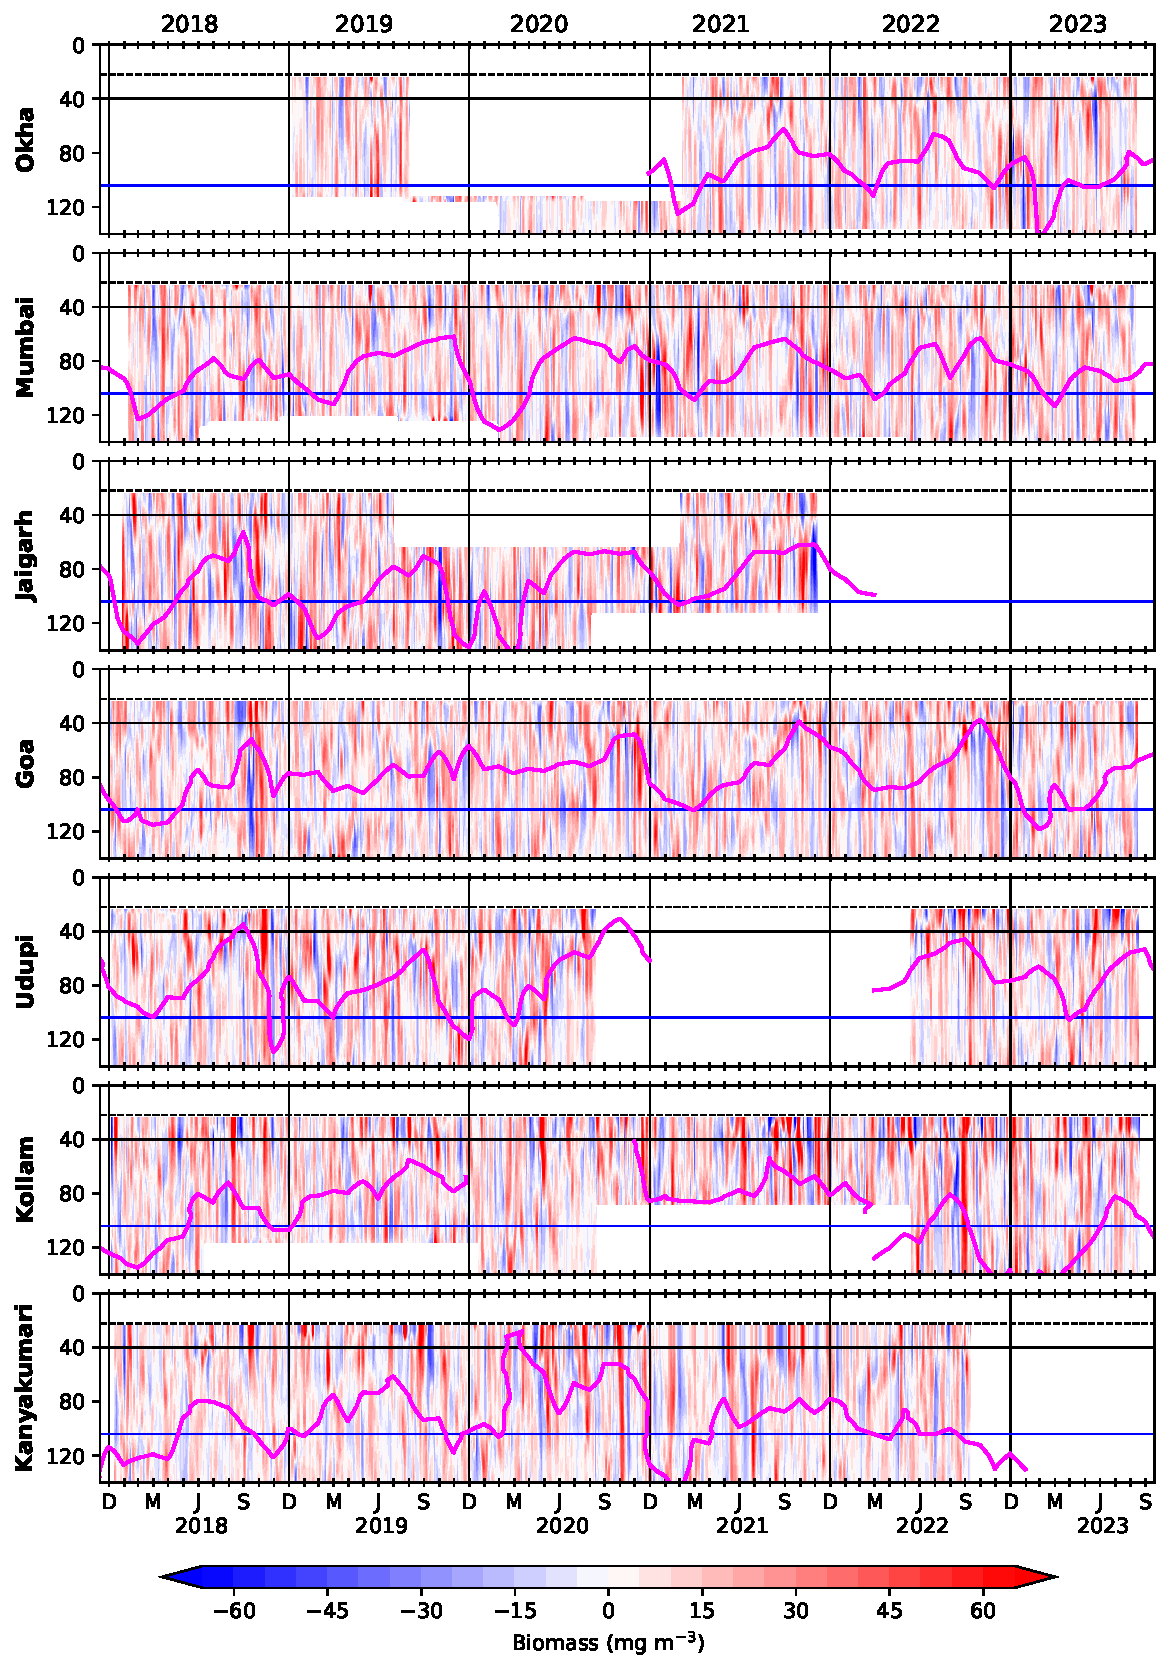
\includegraphics[width=\textwidth]{./figures/filtered_biomass_intraseasonal_5_90days.pdf} 
%	\caption{Biomass variation in intraseasonal band i.e., 5 to 90 days period is obtained using a lanczos band pass filter, It includes both the high- and low-frequency components. The horizontal black and blue lines is for 40 and 104 m, vertical black lines separate the years and solid magenta curves denote $D215$ ($D175$ off Okha and Kanyakumari) fetched from monthly biomass. The dashed line at 22 m marks the top-depth of first bin i.e, 24 m. Intraseasonal variability is seen throughout the record, and it is coherent along the slope, e.g, during October--December 2018.}
%	\label{fig:filtered_biomass_intraseasonal_5_90days_2019}
%\end{figure}

\begin{figure}[htbp]
	\centering
	\includegraphics[width=\textwidth]{./figures/ss_biomass_comparison_intraseasonal_band.pdf} 
	\caption{The 40 and 104 m biomass in comparison with ZSS (column integrated standing stock). The biomass at 104 m may or may not be in phase with upper ocean biomass at 40 m, thereby enhancing or diminishing ZSS variation and it is seen at all the distinct bands of variability.}
	\label{fig:40_104_biomass_zss}
\end{figure}

\begin{figure}[htbp]
		\centering
		\includegraphics[width=0.8\textwidth]{./figures/biomass_intra_2019_kanyakumari.pdf} 
		\caption{Panel of plots showing comparison of variability in seasonal and intraseasonal band off Kanyakumari. The first two panel shows time vs depth plot of seasonal and intraseasonal biomass in same scale: 40 (104) m depths are marked by black (blue) lines, and vertical Grey line separate months, magenta curve shows D175. The third panel from top shows 40 and 104 m daily, intraseasonal (5--90 days), and seasonal (100- 400 days) biomass, mean of daily biomass for respective depth is shown in bottom right of the panel. The fourth panel represents the daily biomass overlaid by 5 day low-pass filtered biomass and daily SLA. Notice the high (low) SLA coinciding with lower (higher) 40 m biomass. The fifth panel shows the difference between daily and 5 day low-pass filtered biomass at 40 and 104 m, Grey (light Grey) shaded region highlights SD (2SD) region of backscatter-biomass equation onto which the daily Chl-\textit{a} is overlaid. The bottom-most panel shows the Chl-\textit{a} and ZSS in Intraseasonal and seasonal band.}		
		\label{fig:biomass_intra_2019_kanyakumari}

\end{figure}

\begin{figure}[htbp]
	\centering
	\includegraphics[width=0.8\textwidth]{./figures/biomass_intra_2019_udupi.pdf} 
	\caption{Same as in Fig.~\ref{fig:biomass_intra_2019_kanyakumari} but for Udupi with D215 curve in top two panels.}		
	\label{fig:biomass_intra_2019_udupi}
\end{figure}

\begin{figure}[htbp]
	\centering
	\includegraphics[width=0.8\textwidth]{./figures/biomass_intra_2019_goa.pdf} 
	\caption{Same as in Fig.~\ref{fig:biomass_intra_2019_kanyakumari} but for Goa with D215 curve in top two panels.}		
	\label{fig:biomass_intra_2019_goa}
\end{figure}


\begin{figure}[htbp]
	\centering
	\includegraphics[width=0.8\textwidth]{./figures/biomass_intra_2019_jaigarh.pdf} 
	\caption{Same as in Fig.~\ref{fig:biomass_intra_2019_kanyakumari} but for Jaigarh with D215 curve in top two panels.}		
	\label{fig:biomass_intra_2019_jaigarh}
\end{figure}

\begin{figure}[htbp]
	\centering
	\includegraphics[width=0.8\textwidth]{./figures/biomass_intra_2019_mumbai.pdf} 
	\caption{Same as in Fig.~\ref{fig:biomass_intra_2019_kanyakumari} but for Mumbai with D215 curve in top two panels.}		
	\label{fig:biomass_intra_2019_mumbai}
\end{figure}

\begin{figure}[htbp]
	\centering
	\includegraphics[width=0.8\textwidth]{./figures/biomass_intra_2019_okha.pdf} 
	\caption{Same as in Fig.~\ref{fig:biomass_intra_2019_kanyakumari} but for Okha with D175 curve in top two panels.}		
	\label{fig:biomass_intra_2019_okha}
\end{figure}


\begin{figure}[htbp]
	\centering
	\includegraphics[width=\textwidth]{./figures/Kollam_2020_verification.pdf} 
	\caption{The \DIFdelbeginFL \DIFdelFL{40 and 104 m }\DIFdelendFL \DIFaddbeginFL \DIFaddFL{top panel shows the hourly }\DIFaddendFL biomass \DIFdelbeginFL \DIFdelFL{in comparison }\DIFdelendFL \DIFaddbeginFL \DIFaddFL{off Kollam, }\DIFaddendFL with \DIFdelbeginFL \DIFdelFL{ZSS }\DIFdelendFL \DIFaddbeginFL \DIFaddFL{the retrieval }\DIFaddendFL (\DIFdelbeginFL \DIFdelFL{column integrated standing stock}\DIFdelendFL \DIFaddbeginFL \DIFaddFL{dashed black line) and deployment (dashed magenta line}\DIFaddendFL ) \DIFaddbeginFL \DIFaddFL{events marked in October 2019 and December 2020, respectively}\DIFaddendFL . The \DIFaddbeginFL \DIFaddFL{bottom left panel presents in-situ }\DIFaddendFL biomass \DIFdelbeginFL \DIFdelFL{at 104 m may or may not be in phase with upper ocean }\DIFdelendFL \DIFaddbeginFL \DIFaddFL{profiles (Bm) as solid lines and corresponding backscatter profiles (Bs) as dashed lines for the pre-retrieval (PR) and post-deployment (PD) phases of 2019 and 2020. The bottom right panel displays }\DIFaddendFL biomass \DIFdelbeginFL \DIFdelFL{at 40 m, thereby enhancing or diminishing ZSS variation }\DIFdelendFL \DIFaddbeginFL \DIFaddFL{(log$_{10}$ scale) plotted against backscatter for Kollam in 2019 }\DIFaddendFL and \DIFdelbeginFL \DIFdelFL{it is seen at }\DIFdelendFL \DIFaddbeginFL \DIFaddFL{2020, overlaid on the linear regression line fitted to }\DIFaddendFL all \DIFaddbeginFL \DIFaddFL{available data points. Symbols used in this panel match those in }\DIFaddendFL the \DIFdelbeginFL \DIFdelFL{distinct bands of variability}\DIFdelendFL \DIFaddbeginFL \DIFaddFL{bottom left panel}\DIFaddendFL .}
	\label{fig:kollam_verification_2020}
\end{figure}

\begin{figure}[htbp]
	\centering
	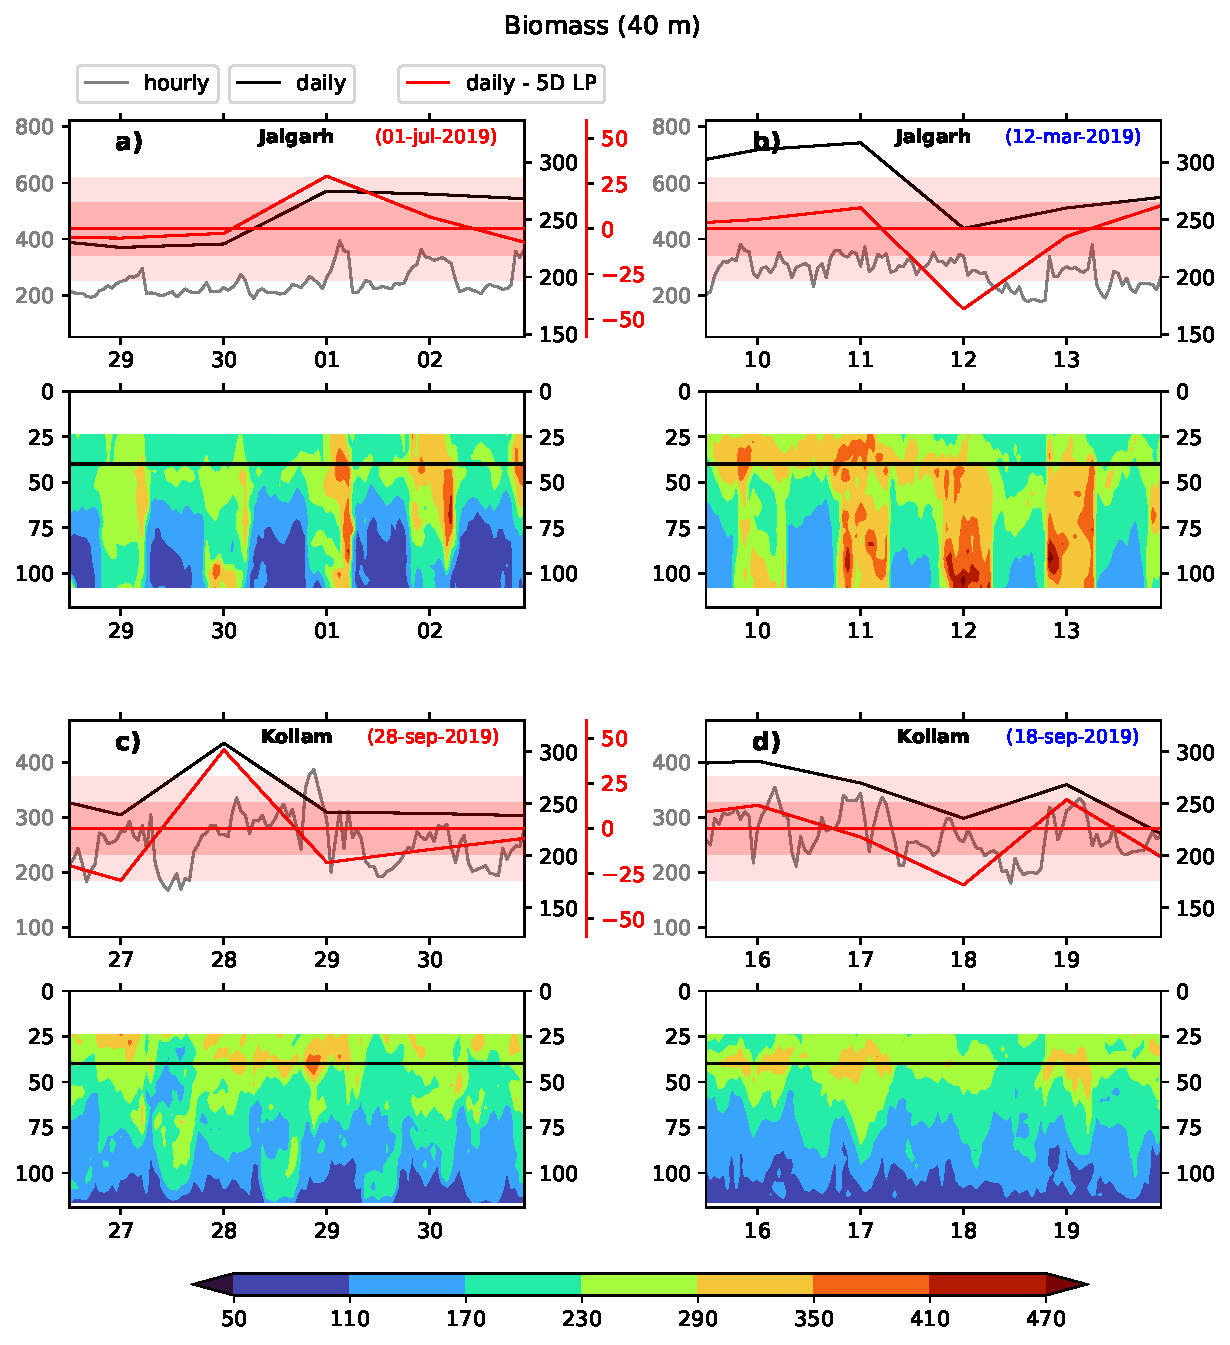
\includegraphics[width=\textwidth]{./figures/biomass_spikes_40m.pdf} 
	\caption{Spikes are shown as the difference between the mean-removed daily biomass time series (red line) and the 5-day low-pass filtered biomass (black line) at 40 m depth, off Jaigarh and Kollam. The overlaid hourly time series illustrates the actual biomass variation throughout the day. Shaded regions represent ±1 SD(red) and ±2 SD (light red) from the mean-removed daily time series. The date of spike occurrence is noted in the top-right corner of each panel, with red and blue text indicating positive and negative spikes, respectively.}
	\label{fig:biomass_spike_40m}
\end{figure}

\begin{figure}[htbp]
	\centering
	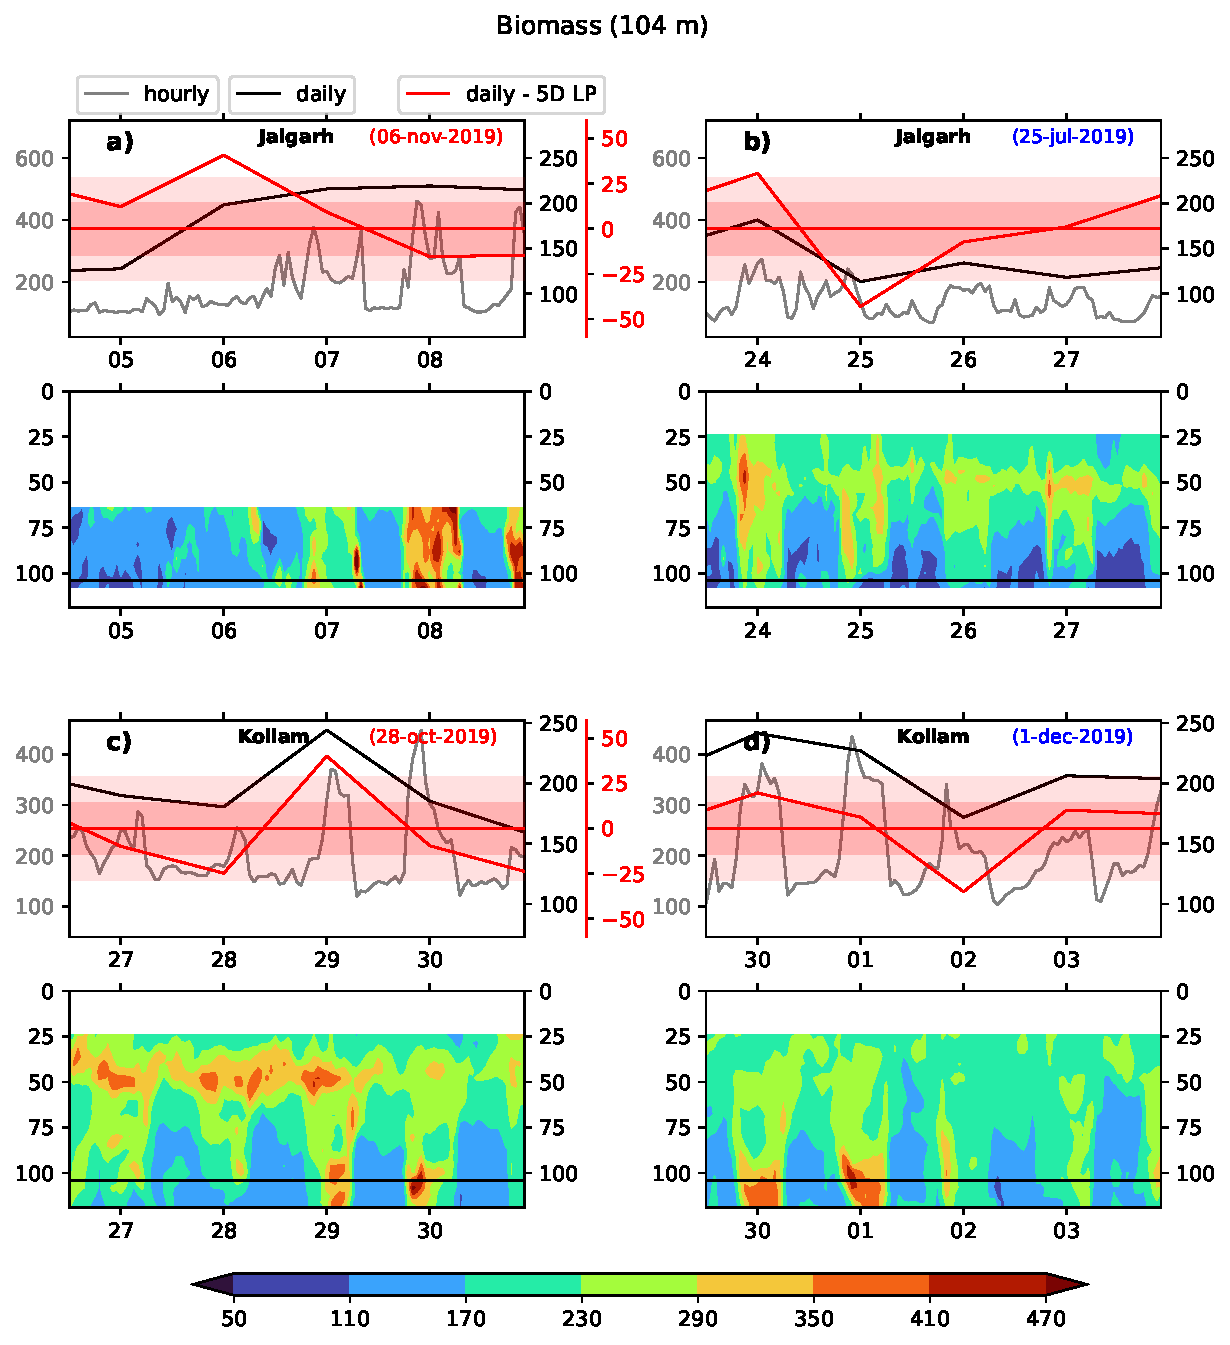
\includegraphics[width=\textwidth]{./figures/biomass_spikes_104m.pdf} 
	\caption{Same as Fig.~\ref{fig:biomass_spike_40m} but for biomass at 104 m depth.}
	\label{fig:biomass_spike_104m}
\end{figure}


\end{document}
